\section{MATERIAL PROPERTIES AND PHYSICAL MODELS}
\normalsize{One of the crucial point of this task are the material properties such as the thermal and mechanical properties and behavior. Those properties can have a big influence on the results of the calculations and they need to be carefully set to accurately model the real life metarial. As is in real life, the material properties are often nonlinear, adding complexity to the calculations.}
\\
\break
\normalsize{\indent The first set of material properties used in early analyses were the ones used by J. Zhu in his 2019 parametric analyses \cites{zhu_parametric_2019} of the \acrshort{ECRH} reflector tile. The properties included the ones for: 
\begin{itemize}
    \item \acrlong{TZM} for the reflector tile.
    \item \acrlong{CuCrZr} for the heat sink.
    \item \acrlong{SS} 1.4981 $X8CrNiMoNb$ for the cooling pipe.
    \item \acrlong{Sigraflex} for the thermal gasket between the heat sink and the reflector tile.
  \end{itemize}
A few of these material properties were based on outdated sources and needed reevalutation to take into account any change.}
\\
\break
\begin{figure}[h!]
    \label{fig_4_1_0} 
    \centering
    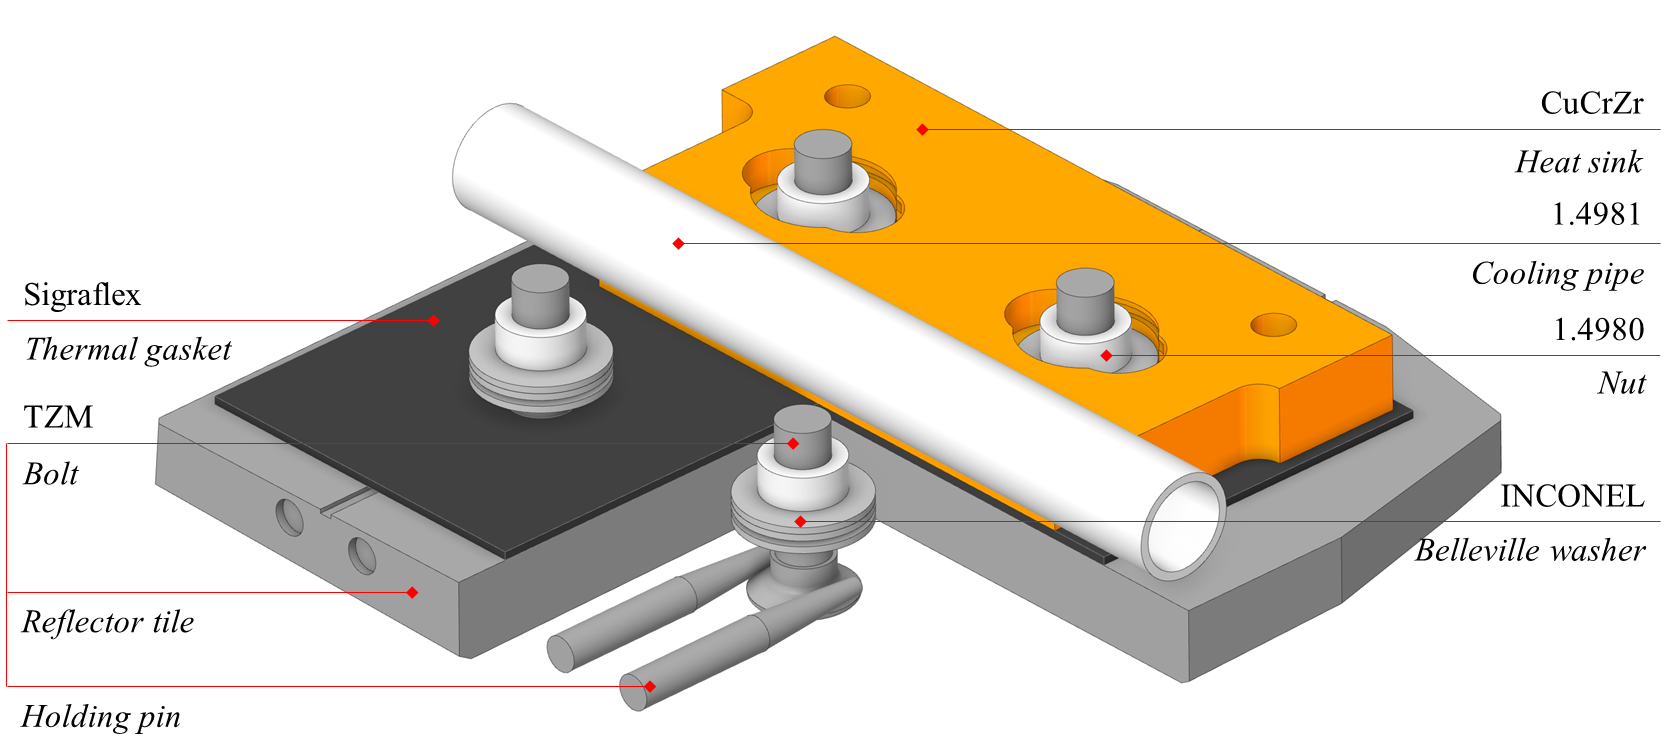
\includegraphics[width=1\textwidth]{figures/materialsforpartsII.png}
    \caption{\it Material assignation}
\end{figure}
\\
\break
\normalsize{\indent The new material properties were set during the project and are split into two big categories, the thermal/physical properties and the mechanical properties. This new set was then saved in an $.xml$ file to be ported to other ANSYS Workbench\textsuperscript{\textregistered} projects (ie. thermal-structural analysis of \acrlong{NBI} target tile).}

\subsection{Thermal properties}
\normalsize{Thermal analysis is the main type of analysis done to evaluate the performances and behavior of the \acrshort{TZM} reflector tile and tile assembly. This is why an accurate modelling of the assembly's constitutive materials is crucial. In addition to the first four materials, the new model should implement the bolting system comprised of \acrshort{TZM} bolts and holding pins, 1.4980 $X5NiCrTi$ \acrshort{SS} nuts and $2.4668$ Inconel Belleville washers. The bolting system was not included in the 2019 model of J. Zhu \cites{zhu_parametric_2019}. Understanding the impact of such bolting system is important to fully analyse the tile. The complete list for thermal properties is (after update):
\begin{itemize}
    \item \acrlong{TZM} for the reflector tile, bolts and holding pins
    \item \acrlong{CuCrZr} for the heat sink.
    \item \acrlong{SS} 1.4981 $X8CrNiMoNb$ for the cooling pipe.
    \item \acrlong{Sigraflex} for the thermal gasket between the heat sink and the reflector tile.
    \item \acrlong{SS} 1.4980 $X5NiCrTi$ for the nuts.
    \item $2.4668$ Inconel for the Belleville washers.
  \end{itemize}
}
\normalsize{\indent It is also important to note that phenomena such as thermal activation and recrystallization of the alloys are NOT taken into account although finite element analysis could technically support such calculations. The implementation of such physical phenomena would require more material data and more ressources in order to correctly model them. It was simply decided to avoid ($if \ possible$) reaching the recrystallization temperatures of the different part material (in particular the maximum temperature of the \acrshort{CuCrZr} heat sink since it is the part that was would overheat \cites{zhu_parametric_2019}{Fellinger_2013}).}
\subsection{Mechanical properties}
\normalsize{Mechanical analysis is the second analysis type that will be carried out to evaluate the structural integrity of the reflector tile assembly. Structural analyses are more complex than thermal analyses and require most computing power. They also heavily depend on the meshing and the modelling of the material (ie. plasticity, elasticity) can greatly influence the results. This is why the choice of the material model is pertinent. In his 2019 study, J. Zhu analyzed the fatigue cycle of the reflector tile assembly \cites{zhu_parametric_2019}. The fatigue criteria will not be used in this study.}
\\
\break
\normalsize{\indent Hardening and plasticity of the material will only be used in special cases (notably for the \acrshort{CuCrZr} alloy) to assess the plastic deformation of the parts. For most, the hardening law will be perfectly plastic (tangent modulus = 0 [$GPA$]) and it was assumed (as a first approach) that the parts shouldn't deform plastically.}
\\
\break
\normalsize{\indent After reading different datasheets and suppliers data, the mechanical properties were reevaluated and condensed into a new revised material database. For the \acrlong{SS} 1.4981 $X8CrNiMoNb$ of the cooling pipe, the mechanical properties were not given and another similar alloy, in particular 1.4435, was used for its mechanical properties ONLY. For other materials such has \acrshort{Sigraflex}, the material data was very limited for lack of supplier's data of a better characterization of it.}
\\
\break
\normalsize{\indent The updated thermal and mechanical properties of the materials are given in tables.}
\begin{table*}\centering
    \ra{1.3}
    \begin{tabular}{@{}rccccccccccc@{}}\toprule
    $T$ & $\lambda$ & $\alpha$ & $C_p$ & $E$ & $\nu$ & $\rho$\\
    \cmidrule{1-7}
    $[\si{\degree} C]$ & $[W \ m^{-1} \si{\degree} C^{-1}]$ & $[\si{\degree} C^{-1}]$ & $[J \ kg^{-1} \si{\degree} C^{-1}]$ & $[GPa]$ & $-$ & $[kg m^{-3}]$\\
    \midrule
    20&-&5,30E-06&-&300&0,32&10200\\
    25&122&-&248&-&-&-\\
    100&121&-&255&-&-&-\\
    200&119&5,30E-06&264&-&-&-\\
    400&116&5,40E-06&279&-&-&-\\
    500&-&-&-&260 &0,32&-\\
    600&112&5,60E-06&289&-&-&-\\
    800&109&5,80E-06&299&-&-&-\\
    1000&-& 6,00E-06&-& 220 &0,32&-\\
    1200&-& 6,20E-06&-&-&-&-\\
    1400&-& 6,40E-06&-&-&-&-\\
    1500&-&-&-&140&0,32&-\\
    2000&-&-&-&40&0,32&-\\
\bottomrule
\end{tabular}
\caption{Thermal and mechanical properties of \acrlong{TZM}}
\end{table*}

\begin{table*}\centering
    \ra{1.3}
    \begin{tabular}{@{}rccccccccccc@{}}\toprule
    $T$ & $\lambda$ & $\alpha$ & $C_p$ & $E$ & $\nu$ & $\rho$\\
    \cmidrule{1-7}
    $[\si{\degree} C]$ & $[W \ m^{-1} \si{\degree} C^{-1}]$ & $[\si{\degree} C^{-1}]$ & $[J \ kg^{-1} \si{\degree} C^{-1}]$ & $[GPa]$ & $-$ & $[kg m^{-3}]$\\
    \midrule
    20 & 338 & 1,57E-05 & 388 & 128 & 0,3 & 8920 \\
    100 & 342 & 1,63E-05 & 392 & 125 & 0,3 & - \\
    200 & 350 & 1,70E-05 & 400 & 121 & 0,3 & - \\
    300 & 360 & 1,76E-05 & 410 & 115 & 0,3 & - \\
    400 & 372 & 1,82E-05 & 422 & 109 & 0,3 & - \\
    500 & 387 & 1,86E-05 & 437 & 102 & 0,3 & - \\
    600 & 404 & 1,88E-05 & 454 & - & - & - \\
    700 & 423 & 1,90E-05 & 473 & - & - & - \\
\bottomrule
\end{tabular}
\caption{Thermal and mechanical properties of \acrlong{CuCrZr}}
\end{table*}

\begin{table*}\centering
    \ra{1.3}
    \begin{tabular}{@{}rccccccccccc@{}}\toprule
    $T$ & $\lambda$ & $\alpha$ & $C_p$ & $E$ & $\nu$ & $\rho$\\
    \cmidrule{1-7}
    $[\si{\degree} C]$ & $[W \ m^{-1} \si{\degree} C^{-1}]$ & $[\si{\degree} C^{-1}]$ & $[J \ kg^{-1} \si{\degree} C^{-1}]$ & $[GPa]$ & $-$ & $[kg m^{-3}]$\\
    \midrule
    20 & 13,5 & 1,61E-05 & 472 & 196 & 0,3 & 8010 \\
    100 & 14,9 & 1,67E-05 & 501 & 190 & 0,3 & - \\
    200 & 16,7 & 1,72E-05 & 525 & 182 & 0,3 & - \\
    300 & 18,3 & 1,77E-05 & 532 & 174 & 0,3 & - \\
    400 & 19,8 & 1,81E-05 & 555 & 166 & 0,3 & - \\
    500 & 21,3 & 1,84E-05 & 582 & 158 & 0,3 & - \\
    600 & 22,7 & 1,88E-05 & 604 & 150 & 0,3 & - \\
    700 & 24,2 & 1,91E-05 & 610 & 142 & 0,3 & - \\
    800 & 25,6 & 1,94E-05 & 611 & 134 & 0,3 & - \\
    900 & - & 1,97E-05 & 615 & - & - & - \\
    1000 & - & 2,00E-05 & 641 & - & - & - \\
\bottomrule
\end{tabular}
\caption{Thermal and mechanical properties of \acrlong{SS} 1.4981}
\end{table*}

\begin{table*}\centering
    \ra{1.3}
    \begin{tabular}{@{}rccccccccccc@{}}\toprule
    $T$ & $\lambda$ & $\alpha$ & $C_p$ & $E$ & $\nu$ & $\rho$\\
    \cmidrule{1-7}
    $[\si{\degree} C]$ & $[W \ m^{-1} \si{\degree} C^{-1}]$ & $[\si{\degree} C^{-1}]$ & $[J \ kg^{-1} \si{\degree} C^{-1}]$ & $[GPa]$ & $-$ & $[kg m^{-3}]$\\
    \midrule
    20 & 15 & 1,70E-05 & 460 & 211 & 0,3 & 8000 \\
    100 & - & 1,70E-05 & - & 206 & 0,3 & - \\
    200 & - & 1,75E-05 & - & 200 & 0,3 & - \\
    300 & - & 1,78E-05 & - & 192 & 0,3 & - \\
    400 & - & 1,80E-05 & - & 183 & 0,3 & - \\
    500 & - & 1,82E-05 & - & 173 & 0,3 & - \\
    600 & - & 1,85E-05 & - & 162 & 0,3 & - \\
\bottomrule
\end{tabular}
\caption{Thermal and mechanical properties of \acrlong{SS} 1.4980}
\end{table*}

\begin{table*}\centering
    \ra{1.3}
    \begin{tabular}{@{}rccccccccccc@{}}\toprule
    $T$ & $\lambda$ & $\alpha$ & $C_p$ & $E$ & $\nu$ & $\rho$\\
    \cmidrule{1-7}
    $[\si{\degree} C]$ & $[W \ m^{-1} \si{\degree} C^{-1}]$ & $[\si{\degree} C^{-1}]$ & $[J \ kg^{-1} \si{\degree} C^{-1}]$ & $[GPa]$ & $-$ & $[kg m^{-3}]$\\
    \midrule
    20 & 12 & 1,34E-05 & 440 & 199 & 0,31 & 8200 \\
    100 & 13 & - & - & 195 & 0,31 & - \\
    200 & - & 1,34E-05 & - & 190 & 0,31 & - \\
    300 & - & 1,38E-05 & - & 185 & 0,31 & - \\
    400 & - & 1,41E-05 & - & 179 & 0,31 & - \\
    500 & 19 & - & - & 174 & 0,31 & - \\
    600 & - & 1,47E-05 & - & 167 & 0,31 & - \\
    700 & 23 & - & - & 163 & 0,31 & - \\
    800 & - & 1,64E-05 & - & 149 & 0,31 & - \\
    900 & 27 & - & - & 134 & 0,31 & - \\
    1000 & - & - & - & 120 & 0,31 & - \\
    1100 & - & - & - & 100 & 0,31 & - \\
\bottomrule
\end{tabular}
\caption{Thermal and mechanical properties of INCONEL 2.4668}
\end{table*}

\begin{table*}\centering
    \ra{1.3}
    \begin{tabular}{@{}rccccccccccc@{}}\toprule
    $T$ & $\lambda_X$ & $\lambda_{Y,Z}$ & $\alpha_X$ & $\alpha_{Y,Z}$ & $C_p$ & $E$ & $\nu$ & $\rho$\\
    \cmidrule{1-9}
    $[\si{\degree} C]$ & $[W \ m^{-1} \si{\degree} C^{-1}]$ & $[W \ m^{-1} \si{\degree} C^{-1}]$ & $[\si{\degree} C^{-1}]$ & $[\si{\degree} C^{-1}]$ & $[J \ kg^{-1} \si{\degree} C^{-1}]$ & $[GPa]$ & $-$ & $[kg m^{-3}]$\\
    \midrule
    20 & 3 & 154 & 3,00E-05 & 1,00E-06 & 700 & 0,7 & 0,15 & 1000 \\
    250 & 2,6 & 105 & - & - & - & - & - & - \\
    500 & 2,1 & 82 & - & - & - & - & - & - \\
    750 & 2,1 & 69 & - & - & - & - & - & - \\
    1000 & 2,1 & 61 & - & - & - & - & - & - \\
    1250 & 2,1 & 56 & - & - & - & - & - & - \\
    1500 & 2,1 & 53 & - & - & - & - & - & - \\
    2000 & 2,1 & 51 & - & - & - & - & - & - \\
\bottomrule
\end{tabular}
\caption{Thermal and mechanical properties of \acrlong{Sigraflex}}
\end{table*}
\newpage